\documentclass[aps,pre,twocolumn,superscriptaddress,floatfix]{revtex4-2}
\usepackage{graphicx}
\graphicspath{{figs/}}
\usepackage{amsmath}
\usepackage{booktabs}
\begin{document}
\title{Kinetic and potential energy scaling in vertically vibrated granular beds: ballistic--collisional subdomains and a smooth energy-partition crossover from data-driven dimensional analysis}
\author{GranuSci Autonomous Research Agent}
\affiliation{Autonomous Research Platform}
\date{\today}

\begin{abstract}
How the kinetic and potential energies of a vertically vibrated granular bed scale with vibration strength $\Gamma$, amplitude-to-diameter ratio $a/d$, and fill height $F$ remains open: existing scaling studies address single responses over restricted ranges, and existing phase diagrams are morphological rather than predictive. We combine 516 discrete-element simulations spanning $\Gamma\in[1.25,160]$, $a/d\in[0.25,4]$, $F\in[4,16]$ with data-driven dimensional analysis (smoothed partial derivatives, subtractive clustering, fuzzy $c$-means, per-subdomain power-law fitting). The dimensionless kinetic energy $e_k^*$ admits a compact two-subdomain pure power law: $e_k^*=2.958\,(a/d)^{0.564}\Gamma^{0.717}F^{-0.811}$ (collisional, 278 cases, $\delta=18.0\%$) and $e_k^*=2.059\,(a/d)^{1.044}\Gamma^{0.629}F^{-0.554}$ (ballistic, 106 cases, $\delta=29.4\%$), with global error $\delta^*=21.1\%$ versus $23.5\%$ single-domain. The potential-energy proxy $e_p^*$ (mean elevation in diameters) resists compact partitioning: six subdomains with no stable cluster-count plateau, exponents on $a/d$ flipping from $-0.22$ to $+0.78$ and on $F$ from $-1.05$ to $+0.58$ between neighbors ($\delta^*=26.9\%$ versus $35.9\%$ single-domain). Snapshot and time-averaged field diagnostics at $F=8$ show the two kinetic subdomains differ in energy-injection mechanism---ballistic flight at large $a/d$ or extreme $\Gamma$ (coherent plugging bed or Fermi-accelerated Leidenfrost state with a levitated dense layer above a bottom gap), collisional boiling otherwise---cutting across morphological state categories. The partition ratio $R=e_p^*/(e_k^*+e_p^*)$ varies smoothly along the model line from 0.13 through a 0.60 plateau to 0.90 with increasing $\Gamma$; hold-out measurements at $\Gamma=4$ and 15 straddle the plateau with no discontinuity. Six hold-out simulations validate the kinetic scaling with 16.5\% mean absolute error. Mechanism-resolved subdomains thus replace morphological state labels with quantitative, transferable scaling criteria.
\end{abstract}

\maketitle

\section{Introduction}
\label{sec:intro}
Vertically vibrated granular beds display a rich spectrum of states---solid-like compaction, bouncing beds, undulations, buoyancy-driven convection, the granular Leidenfrost state, and granular gases \cite{jaeger1996,eshuis2007,meerson2005,rivas2015,eshuis2010}. Two complementary descriptions exist. The first is \emph{morphological}: Eshuis \emph{et al.} mapped phase boundaries of a shallow quasi-two-dimensional bed in $(F,\Gamma)$ and $(F,S)$ planes ($S=a^2\omega^2/gd$), identifying detachment, undulation, Leidenfrost, and convection thresholds from direct observation \cite{eshuis2007}. The second is \emph{quantitative scaling}: granular temperature and mean kinetic energy have been reported to scale as powers of peak vibration velocity or $\Gamma$ \cite{zivkovic2011,hsiau2008,bhateja2016}, most often for a single response variable over a restricted parameter range.

Missing is a joint quantitative account of how the two mechanical-energy reservoirs---kinetic and potential---scale across the full parameter space $(\Gamma,a/d,F)$, and whether scaling-regime boundaries coincide with morphological phase boundaries. The question matters beyond taxonomy: industrial vibrated-bed processes are designed by adjusting $\Gamma$, $a$, and fill level, and design rules based on mechanism-resolved energy scaling are more transferable than state labels.

Three unknowns define the gap. First, no prior study jointly fits the dimensionless mean kinetic energy $e_k^*$ and a potential-energy proxy $e_p^*$ (mean particle elevation in particle diameters) over a common parameter space; published scaling laws treat one response at a time \cite{zivkovic2011,hsiau2008}, and the partition between kinetic and potential reservoirs has been described only qualitatively \cite{eshuis2007}. Second, existing phase diagrams report observation-based boundaries \cite{eshuis2007,rivas2015}; whether scaling exponents change abruptly at those boundaries---the signature of a mechanism switch---or vary smoothly is unknown. Third, $a/d$ is known to matter independently of $\Gamma$ \cite{jaeger1996,bhateja2016}, but its interaction with $F$ in multilayer beds is unresolved quantitatively.

We address these unknowns with data-driven dimensional analysis (DDDA): smoothed partial derivatives identify local power-law sensitivities, subtractive clustering with fuzzy $c$-means partitions the exponent field into subdomains, and each subdomain receives a closed-form power law \cite{constantine2014,buckingham1914}. The approach is agnostic to preconceived phase labels and lets the data reveal how many regimes are actually needed. We ran 516 discrete-element simulations covering two decades of $\Gamma$, four octaves of $a/d$, and three fill heights, in an adaptive two-round design with boundary refinement and independent hold-out validation.

This paper contributes: (i) a two-subdomain pure power law for $e_k^*$ whose subdomains differ in exponents on all three parameters; (ii) the demonstration that $e_p^*$ resists compact partitioning---a continuously varying response with sign-flipping sensitivities; (iii) mechanistic identification of the kinetic subdomains as \emph{ballistic} versus \emph{collisional} energy injection, established by snapshots and time-averaged solid-fraction fields at $F=8$, cutting across morphological categories; and (iv) a smooth energy-partition landscape $R(\Gamma,a/d,F)$ with no internal discontinuity.

\section{System and methods}
\label{sec:methods}

\subsection{Simulated system}
We simulate a quasi-two-dimensional cell (length 0.10 m, height 0.20 m, width 4.5 mm) with monodisperse spheres ($d=2$ mm, density 2500 kg/m$^3$) in the LIGGGHTS discrete-element platform. The base executes sinusoidal vertical motion $z_b(t)=a\sin\omega t$. The three dimensionless control parameters are vibration strength $\Gamma=a\omega^2/g$, amplitude-to-diameter ratio $a/d$, and nominal fill height $F$ (rest layers; realized counts 106/231/502 particles for $F=4/8/16$ after gravitational settling). Each run discards 20 development periods and averages over 8 statistical periods.

\subsection{Response variables}
The primary responses are
\begin{equation}
e_k^*=\frac{\langle \tfrac12|\mathbf u|^2\rangle}{gd},\qquad
e_p^*=\frac{\langle y\rangle}{d},
\label{eq:responses}
\end{equation}
the dimensionless mean kinetic energy and the mean particle elevation above the base in units of $d$. Because $e_p^*$ is an elevation rather than a gravitational energy, all partition statements below are statements about the split between elevation and motion on the common scale $gd$. The vertical granular temperature $t_y^*$ and center-of-mass height $h_m^*$ are analyzed for comparison. The partition ratio is $R=e_p^*/(e_k^*+e_p^*)$.

\subsection{Design of simulations}
Round 1: full factorial grid, $\Gamma$ at 15 log-spaced levels in $[1.25,160]$, $a/d$ at 9 log-spaced levels in $[0.25,4]$, $F\in\{4,8,16\}$---405 cases. Round 2: boundary refinement (5 new $a/d$ levels $\times$ 7 new $\Gamma$ levels $\times$ 3 $F$, 105 cases) plus 6 hold-out validation points at $(a/d,\Gamma)=(0.45,4),(0.45,15),(0.85,4),(0.85,15),(1.5,4),(1.5,15)$, $F=8$. Merging all runs and de-duplicating repeated parameter combinations (105 duplicates) leaves 516 unique valid cases: 405 from round 1 and 111 from round 2 (105 refinement plus 6 hold-out, one of which duplicated a refinement point). No case failed.

\subsection{Data-driven dimensional analysis}
DDDA proceeds in three steps. (1) Smoothed partial derivatives $\partial\log Y/\partial\log X_i$ are estimated by adaptive Gaussian-weighted local linear regression in log space. (2) Subtractive clustering (radius factor $r_a$) plus fuzzy $c$-means ($m=2$) partitions the exponent field; points with maximum membership below 0.6 are ambiguous. (3) Each cluster defines a subdomain; within it the composite $C=(a/d)^{D_1}\Gamma^{D_2}F^{D_3}$ follows from the dominant eigenvector, and the physical-space law $Y=A\,C^{b}$ (pure power law, $c=0$) is fitted with iterative residual-based outlier cleaning. The global error metric is
\begin{equation}
\delta^*=\frac1N\sum_i\frac{|Y_i^{\rm pred}-Y_i|}{Y_i}.
\end{equation}
The radius $r_a$ controls resolution; we sweep $r_a\in\{0.2,0.3,0.4,0.5\}$ and require stable cluster counts across neighbors before accepting a partition. Single-cluster fits ($n=1$) provide baselines. Subdomain membership at new points is predicted by 7-nearest-neighbor voting in log space, which also yields interfacial vote fractions.

\section{Results and discussion}
\label{sec:results}

\subsection{Kinetic energy: a robust two-subdomain power law}
\label{sec:ek}
For $e_k^*$ the DDDA partition is stable: at $r_a=0.3$ the merged 516-case dataset resolves two subdomains with global error $\delta^*=21.1\%$, versus $23.5\%$ for a single-domain fit ($e_k^*=2.540\,(a/d)^{0.647}\Gamma^{0.698}F^{-0.700}$, $R^2=0.956$)---a 10\% relative improvement [Fig.~\ref{fig:benefit}(a)]. The subdomain laws are
\begin{align}
\text{subdomain 0 (collisional):}\;\; e_k^*&=2.958\,(a/d)^{0.564}\Gamma^{0.717}F^{-0.811},\label{eq:sub0}\\
\text{subdomain 1 (ballistic):}\;\; e_k^*&=2.059\,(a/d)^{1.044}\Gamma^{0.629}F^{-0.554}.\label{eq:sub1}
\end{align}
Subdomain 0 carries 308 of 516 cases (59.7\%), of which 278 survive outlier cleaning, with $\delta=18.0\%$, $R^2=0.982$; subdomain 1 carries 117 cases (22.7\%), 106 after cleaning, with $\delta=29.4\%$, $R^2=0.810$. The remaining 91 cases (17.6\%) fall below the membership threshold, concentrated in the transition band. The decisive evidence for two subdomains is not the modest error reduction but the \emph{exponent shift}: the $a/d$ exponent nearly doubles ($0.564\to1.044$) while the $\Gamma$ and $F$ exponents change little.

Three checks support Eqs.~(\ref{eq:sub0})--(\ref{eq:sub1}). First, the round-1 fits (405 cases, subdomains of 225 and 109 cases) reproduce the merged-data exponents closely: the subdomain-0 exponents shift by at most $0.03$ ($a/d$: $0.547\to0.564$), while the subdomain-1 $a/d$ exponent shifts by $0.095$ ($0.949\to1.044$) with the $\Gamma$ and $F$ exponents stable to $0.07$ ($0.705\to0.629$, $0.624\to0.554$)---demonstrating insensitivity to boundary refinement at the level of the exponent precision. Second, resolution sweeps show the cluster count is stable at 2 for $r_a=0.3$--$0.4$ while finer radii ($r_a\le0.2$) over-segment. Third, the six hold-out simulations---run after the model was frozen, at $(a/d,\Gamma)$ combinations absent from the training grid---validate the scaling: predictions lie within $-3.2\%$ to $+34.1\%$ of the measurements, with mean absolute error 16.5\% and mean signed error $+15.5\%$ (Fig.~\ref{fig:validation}). The systematic overprediction concentrates at $\Gamma=15$ inside the transition band, consistent with the subdomain interface running between the $\Gamma=4$ and $\Gamma=15$ validation columns.

\begin{figure}[t]
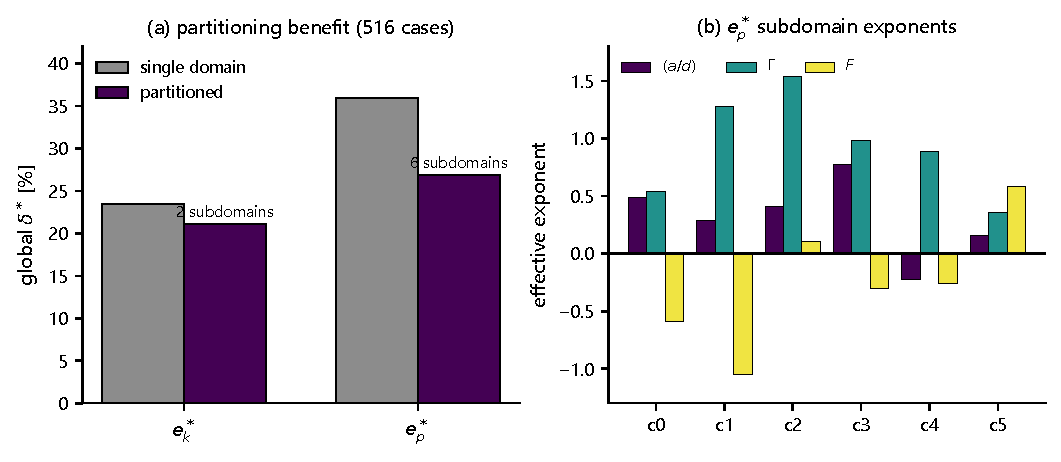
\includegraphics[width=\columnwidth]{fig_26}
\caption{(a) Global relative error $\delta^*$ of single-domain versus partitioned power-law fits on the merged 516-case dataset: $e_k^*$ needs only two subdomains; $e_p^*$ fragments into six with no stable plateau. (b) Effective exponents of the six $e_p^*$ subdomains, showing sign flips on $a/d$ (c4: $-0.221$) and $F$ (c2: $+0.103$, c5: $+0.582$, versus c1: $-1.047$).}
\label{fig:benefit}
\end{figure}

\begin{figure}[t]
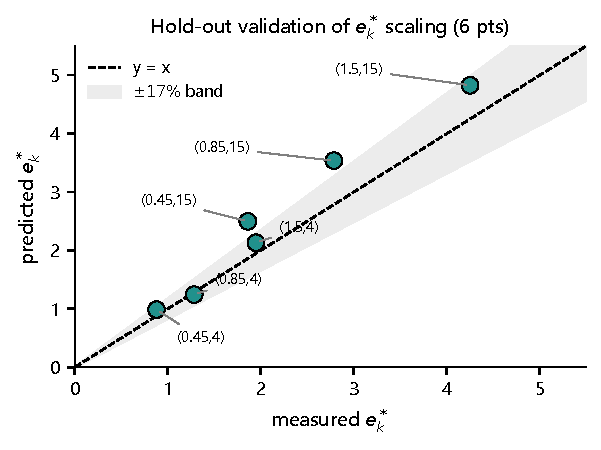
\includegraphics[width=\columnwidth]{fig_20}
\caption{Hold-out validation of the $e_k^*$ scaling. Six independent simulations (labels give $(a/d,\Gamma)$, $F=8$) against predictions from the round-1 model. The shaded band marks $\pm17\%$, the round-1 subdomain error scale; the mean absolute error is 16.5\%.}
\label{fig:validation}
\end{figure}

\subsection{Potential energy: a response that resists partitioning}
\label{sec:ep}
The potential-energy proxy $e_p^*$ behaves qualitatively differently. At every resolution the optimal partition splinters: $r_a=0.3$ gives 11 clusters ($\delta^*=24.5\%$, 48\% ambiguous), $r_a=0.4$ gives 6 clusters ($\delta^*=26.9\%$, 35.5\% ambiguous), $r_a=0.5$ gives 5 clusters ($\delta^*=21.2\%$, 28.6\% ambiguous, on the 405-case round-1 data). No stable plateau exists in the cluster count, and the six-cluster solution orders exponents non-monotonically across neighboring clusters [Fig.~\ref{fig:benefit}(b)]: the $a/d$ exponent ranges from $-0.221$ (c4) to $+0.778$ (c3), the $F$ exponent from $-1.047$ (c1) to $+0.582$ (c5). The single-domain baseline is poor ($\delta^*=35.9\%$, $R^2=0.829$), so partitioning helps by 25\% relative, but no compact law emerges.

The physical reading is that $e_p^*$ varies by smooth crossover rather than by switching between a few mechanisms. The smoothed derivative field makes this explicit: the local $a/d$ sensitivity spans $[-0.675,+1.534]$ and the local $F$ sensitivity spans $[-1.432,+0.812]$, with sign changes along continuous fronts rather than at isolated boundaries. Increasing $a/d$ raises the bed at moderate $\Gamma$ but lowers the mean elevation in the deep-bed low-$\Gamma$ corner (cluster 4's negative $a/d$ exponent: thick beds loft less per unit drive); increasing $F$ raises the mean elevation at low $\Gamma$ (cluster 5's positive $F$ exponent) but lowers it in the strongly agitated regime (cluster 1: energy diluted among more particles). These opposing trends superpose and interpolate, defeating low-dimensional partitioning.

The contrast between $e_k^*$ (two clean subdomains) and $e_p^*$ (no compact partition) is itself a result: the two reservoirs sample the mechanism landscape differently. Kinetic energy is set by the injection mechanism at the bed base, which switches sharply between ballistic and collisional regimes; potential energy integrates the entire bed-height distribution, which deforms continuously as the bed fluidizes and expands.

\subsection{Subdomain geometry and the failure of single-parameter criteria}
\label{sec:geometry}
Where does the $e_k^*$ boundary run? Probing the trained classifier on a $(a/d,\Gamma)$ grid at $F=8$ (Fig.~\ref{fig:geometry}) shows subdomain 1 (ballistic) occupying two opposite corners: large $a/d$ at low $\Gamma$ ($a/d\gtrsim0.6$, $\Gamma\lesssim5$) and small $a/d$ at extreme $\Gamma$ ($a/d\lesssim0.3$, $\Gamma\gtrsim80$). Subdomain 0 (collisional) fills the diagonal band between, including the whole $a/d=0.25$ column up to $\Gamma\approx40$ and the whole $\Gamma=20$ row. Along $F$, the boundary moves monotonically: at fixed $(a/d,\Gamma)=(0.25,1.25)$, $F=4$ belongs to subdomain 0 while $F=16$ belongs to subdomain 1, and likewise at $(1.0,2.5)$ and $(2.0,5.0)$---deep beds stay solid-like to higher $\Gamma$, consistent in trend with the Rayleigh--Janssen detachment criterion $\Gamma_{\rm detach}=2-e^{-\chi}$, whose critical value rises with bed depth \cite{eshuis2007}.

Two features deserve emphasis. First, the interface is \emph{diffuse}: at boundary points the 7-nearest-neighbor votes split (4:3 at $a/d=1$, $\Gamma=5$ and 80), and 17.6\% of cases fall below the membership threshold. Second, the boundary is \emph{not} a single-parameter criterion: constant-$\Gamma$ lines fail (the boundary spans $\Gamma\approx2.5$ to beyond 160), and constant-$\Gamma(a/d)^p$ lines also fail, as shown by the negative-slope guides in Fig.~\ref{fig:geometry}, which run opposite to the corner-shaped interface. The two-parameter structure reflects the two distinct routes into the ballistic regime documented next.

\begin{figure}[t]
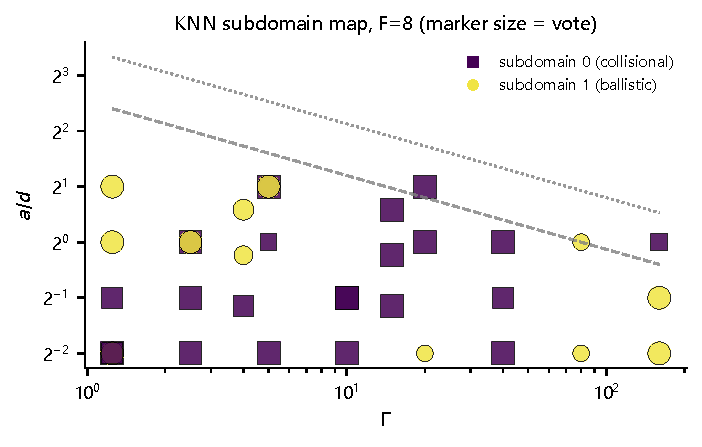
\includegraphics[width=\columnwidth]{fig_18}
\caption{Subdomain membership map for $e_k^*$ in the $(\Gamma,a/d)$ plane at $F=8$, probed by 7-neighbor voting on the trained DDDA classifier. Squares: subdomain 0 (collisional); circles: subdomain 1 (ballistic); marker size encodes the majority vote fraction (small markers = interfacial). Gray dashed/dotted lines: constant-$\Gamma(a/d)^{2.5}$ guides, drawn to show that no single power-law criterion matches the corner-shaped boundary.}
\label{fig:geometry}
\end{figure}

\subsection{Mechanism: ballistic versus collisional injection at $F=8$}
\label{sec:mechanism}
Snapshot and field diagnostics at $F=8$ (231 particles) resolve what the subdomains mean physically (Fig.~\ref{fig:snapshots}). The subdomain-1 case at $(a/d,\Gamma)=(1,2.5)$ is a solid-like plug: a dense bed with flat surface (top at 12--15 mm), particle velocities uniform at 0.1--0.3 m/s---of the order of the base velocity scale $\sqrt{\Gamma g a}\approx0.22$ m/s---with a few fast particles at the base absorbing the landing impact. The bed takes off and lands as a body; its kinetic energy is \emph{coherent translational} energy set by the base velocity. The subdomain-0 case at $(1,40)$ is a collisional boiling bed: a dense phase topped by a dilute spray, collision hot spots (0.7--1.1 m/s) at the base, a few particles launched 2--3 diameters above the surface; energy dissipates through inelastic collisions within the bed.

The other route into subdomain 1, at $(0.25,160)$, looks morphologically completely different---a dispersed cloud filling about three quarters of the cell---yet the time-averaged solid-fraction field (Fig.~\ref{fig:field}) shows a levitated layer (peak horizontally averaged fraction 0.09 at $y=18$ mm) above a 12-mm bottom gap, with plume-like streaks rising to a cloud top of 116 mm: a granular Leidenfrost state \cite{meerson2005,rivas2015}. Particle speeds in the snapshot span 0.1--1.0 m/s, with the fastest particles in the dilute top spray, consistent with launch speeds of order the base velocity scale $\omega a\approx0.89$ m/s---a Fermi-like acceleration picture \cite{eshuis2007,meerson2005}. For comparison, the $F=4$ case at the same $(a/d,\Gamma)$ shows the same structure with a slightly thicker gap ($\sim$20 mm) and higher levitated peak (fraction 0.08 at $y=25$ mm), so the Leidenfrost morphology is robust across fill heights in this corner of parameter space.

\begin{figure}[t]
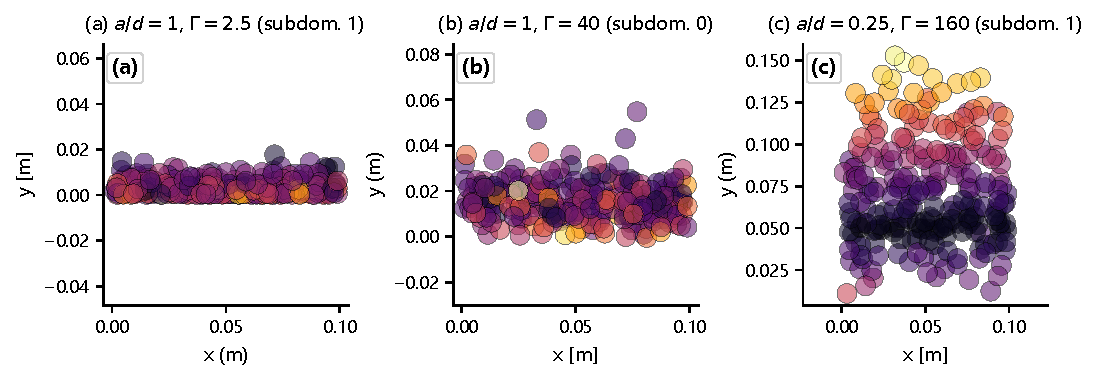
\includegraphics[width=\columnwidth]{fig_29}
\caption{End-frame snapshots colored by particle speed for three representative $F=8$ cases (231 particles each): (a) $(a/d,\Gamma)=(1,2.5)$, subdomain 1---coherent plugging bed (ballistic, solid-like); (b) $(1,40)$, subdomain 0---collisional boiling bed with dilute spray; (c) $(0.25,160)$, subdomain 1---dispersed granular gas / Leidenfrost state (ballistic, gas-like). Panels (a) and (c) share a scaling subdomain despite opposite morphology.}
\label{fig:snapshots}
\end{figure}

\begin{figure}[t]
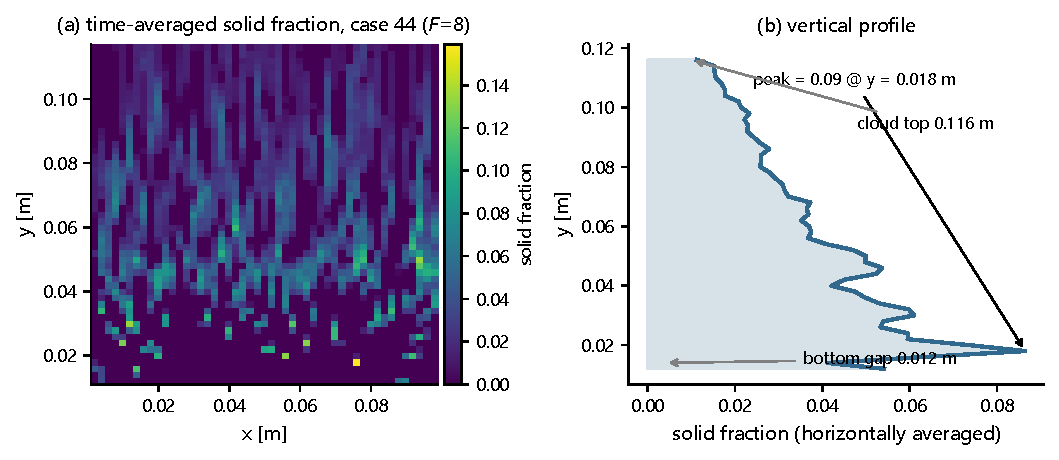
\includegraphics[width=\columnwidth]{fig_28}
\caption{Time-averaged solid-fraction field (a) and horizontally averaged vertical profile (b) for the Leidenfrost case $(a/d,\Gamma)=(0.25,160)$, $F=8$. A 0.012 m gap separates the base from a levitated layer peaking at 0.09 near $y=0.018$ m; above a shoulder near $y=0.04$--$0.05$ m the profile decays monotonically to a cloud top at 0.116 m.}
\label{fig:field}
\end{figure}

The mechanistic unification rests on the $a/d$ exponent. In a ballistic regime the particle velocity inherits the base velocity scale $v\sim\omega a=\sqrt{\Gamma g a}$, so $e_k^*\propto(\omega a)^2/(gd)\propto\Gamma\,(a/d)$ at fixed $F$: unit $a/d$ and unit $\Gamma$ exponents before dilution among layers. Subdomain 1 matches the unit $a/d$ exponent closely ($1.044$), while its $\Gamma$ exponent ($0.629$) falls well below unity---consistent with partial dissipation of the injected energy, and with the $F$ dilution factor ($F^{-0.554}$) absorbing part of the depth dependence; the ballistic identification therefore rests on the $a/d$ exponent and the direct velocity evidence, not on a full unit-exponent match. In a collisional regime the bed stays dense, collisions randomize the energy, and the drive enters through a dissipation balance, softening the $a/d$ exponent to 0.564. The subdomains thus classify \emph{energy-injection mechanisms}, not morphological states: the plugging bed [Fig.~\ref{fig:snapshots}(a)] and the Leidenfrost cloud [Fig.~\ref{fig:snapshots}(c)] sit in one subdomain because both feed energy ballistically from the base, while the boiling bed [Fig.~\ref{fig:snapshots}(b)] thermalizes it collisionally. This explains why the $e_k^*$ boundary cuts across the morphological phase diagram of Eshuis \emph{et al.} \cite{eshuis2007} rather than retracing it, and why single-parameter criteria fail.

As a caveat, the exponent identification rests on fits with $\delta\sim18$--29\%; the ballistic interpretation of subdomain 1 is favored by the snapshot and field evidence and by the near-unit $a/d$ exponent, but a dedicated study varying material dissipation would be needed to close the mechanism quantitatively.

\subsection{Energy partition: a smooth crossover landscape}
\label{sec:partition}
Combining both response models yields the partition ratio $R=e_p^*/(e_k^*+e_p^*)$ (Fig.~\ref{fig:partition}). Along the model line $a/d=0.5$, $F=8$, $R$ rises from 0.133 at $\Gamma=2.5$ (kinetic-dominated coherent bouncing) through a plateau of $\approx0.60$ at $\Gamma=10$--$40$ (collisional regime, the two reservoirs sharing the injected energy roughly equally) to 0.896 at $\Gamma=160$ (potential-dominated Leidenfrost state, the bed lofted high).

The hold-out measurements probe the partition at two $\Gamma$ values, 4 and 15, for three $a/d$ values each. Pairwise at fixed $a/d$, $R$ \emph{decreases} from $\Gamma=4$ to $\Gamma=15$ (from 0.707 to 0.645 at $a/d=0.45$; from 0.669 to 0.616 at $0.85$; from 0.635 to 0.578 at $1.5$)---opposite in sign to the model line's shallow rise ($<0.05$ in $R$) over the same interval. The measured values (0.578--0.707) straddle the model plateau ($\approx0.60$): the two $\Gamma$ columns bracket the plateau from both sides, and the measured dip (0.05--0.06 in $R$) is comparable to the scatter expected from the subdomain fit errors ($\delta\sim18$--29\%). We therefore do not claim a confirmed monotone $\Gamma$ trend from the hold-out data; what they support is (i) the absence of any discontinuity in $R$ across the transition band, and (ii) the level of the plateau. Within each $\Gamma$ column, smaller $a/d$ gives larger $R$, consistent with the model's depth trend (deeper relative beds store more of their energy in elevation).

\begin{figure}[t]
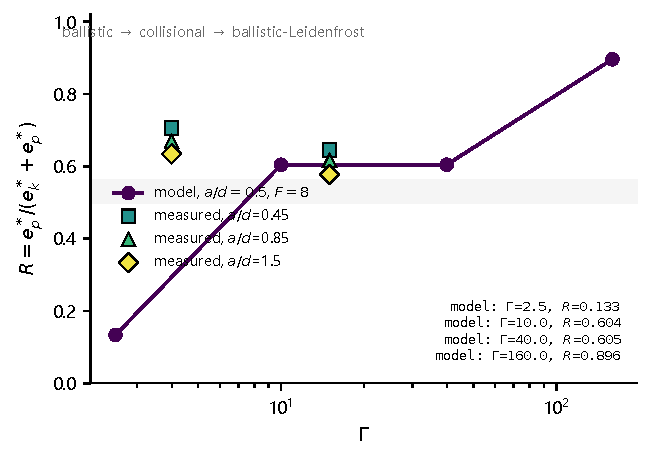
\includegraphics[width=\columnwidth]{fig_25}
\caption{Energy-partition ratio $R=e_p^*/(e_k^*+e_p^*)$ versus $\Gamma$. Line with circles: model prediction at $a/d=0.5$, $F=8$ (from the subdomain power laws); symbols: hold-out measurements at $a/d=0.45$, $0.85$, $1.5$, $F=8$. The model line crosses from kinetic-dominated ($R\approx0.13$) through a $\approx0.6$ plateau to potential-dominated ($R\approx0.9$); the hold-out pairs at $\Gamma=4$ and 15 straddle the plateau level with no discontinuity.}
\label{fig:partition}
\end{figure}

The partition landscape contains no jump. $R$ varies smoothly across the parameter space, fully consistent with the non-partitionability of $e_p^*$ (Sec.~\ref{sec:ep}): both reservoirs deform continuously, and only the kinetic reservoir carries a signature of the ballistic--collisional switch. For applications this means the split of drive energy between agitation and lofting is a smoothly varying function of $(\Gamma,a/d,F)$ in this range, while the \emph{character} of the agitation (coherent versus thermal) switches more sharply along the subdomain interface.

\section{Conclusions}
\label{sec:conclusions}
We mapped the joint kinetic--potential energy scaling of a vertically vibrated granular bed over $\Gamma\in[1.25,160]$, $a/d\in[0.25,4]$, $F\in[4,16]$ using 516 discrete-element simulations and data-driven dimensional analysis. The kinetic energy $e_k^*$ follows a two-subdomain pure power law [Eqs.~(\ref{eq:sub0})--(\ref{eq:sub1})], validated on six hold-out cases to 16.5\% mean absolute error; the subdomains correspond to ballistic and collisional energy injection---identified through the near-unit $a/d$ exponent (1.044) plus direct velocity evidence---a mechanism-based boundary cutting across morphological phase categories and defeating single-parameter criteria. The potential-energy proxy $e_p^*$ resists compact partitioning, with $a/d$ and $F$ sensitivities that flip sign along continuous fronts; the energy partition $R$ consequently varies smoothly from 0.13 to 0.90 along the model line with no discontinuity, the hold-out pairs bracketing the mid-range plateau. These results replace morphological state labels with a two-layer description: a sharp switch in injection mechanism (kinetic energy) embedded in a continuous crossover landscape (energy partition).

Limitations bound the claims. All results hold for one material parameter set (fixed restitution and friction) and one quasi-two-dimensional geometry; material-parameter sweeps were outside our tool's reach and remain open. The potential-energy proxy is a mean elevation, not the full gravitational-energy distribution. Transition-band statistics rest on 8-period averaging, and interfacial points show vote splitting, so boundary locations carry $\mathcal O(10\%)$ uncertainty. The mechanism interpretation of the ballistic subdomain rests on the $a/d$ exponent and snapshot/field evidence at three representative cases; direct dissipation-budget measurements are needed to close it quantitatively. Future work should test whether the ballistic $a/d$ exponent stays near unity under restitution changes, and whether the $R$ plateau at $\approx0.6$ is universal or material-dependent.

\begin{thebibliography}{99}

\bibitem{jaeger1996} H.~M. Jaeger, S.~R. Nagel, and R.~P. Behringer, Granular solids, liquids, and gases, Rev. Mod. Phys. \textbf{68}, 1259 (1996).

\bibitem{eshuis2007} P.~Eshuis, K.~van der Weele, D.~van der Hoef, M.~Alder, and D.~Lohse, Phase diagram of vertically shaken granular matter, Phys. Fluids \textbf{19}, 123301 (2007).

\bibitem{meerson2005} B.~Meerson, T.~P\"oschel, and Y.~Bronfman, The granular Leidenfrost effect: experiment and theory of floating particle clusters, Phys. Rev. Lett. \textbf{95}, 258001 (2005).

\bibitem{rivas2015} N.~Rivas \emph{et al.}, From the granular Leidenfrost state to buoyancy-driven convection, Phys. Rev. E \textbf{91}, 042202 (2015).

\bibitem{eshuis2010} P.~Eshuis, K.~van der Weele, D.~van der Hoef, and D.~Lohse, Onset of convection in strongly shaken granular matter, Phys. Rev. Lett. \textbf{104}, 038001 (2010).

\bibitem{zivkovic2011} V.~Zivkovic, M.~J. Biggs, and D.~H. Glass, Scaling of granular temperature in a vibrated granular bed, Phys. Rev. E \textbf{83}, 031308 (2011).

\bibitem{hsiau2008} S.~S. Hsiau, L.~S. Lu, and C.~H. Tai, Experimental investigations of granular temperature in vertical vibrated beds, Powder Technol. \textbf{182}, 132 (2008).

\bibitem{bhateja2016} A.~Bhateja and D.~V. Khakhar, Vibrated granular bed: scaling of mean granular temperature, Phys. Rev. E \textbf{94}, 042901 (2016).

\bibitem{constantine2014} P.~G. Constantine, E.~Dow, and Q.~Wang, Active subspace methods in theory and practice: applications to kriging surfaces, SIAM J. Sci. Comput. \textbf{36}, A1500 (2014).

\bibitem{buckingham1914} E.~Buckingham, On physically similar systems; illustrations of the use of dimensional equations, Phys. Rev. \textbf{4}, 345 (1914).

\end{thebibliography}

\end{document}